\documentclass[usenames,dvipsnames]{beamer}

\usepackage{tikz}
\usepackage{amsmath}
\usepackage{listings}
\usepackage{graphicx}
\usepackage{inconsolata}
\usepackage{epigraph}
\usepackage[backend=biber,style=numeric-comp,sorting=none]{biblatex}
\usetheme{LANL}
\usetikzlibrary{positioning, shapes.misc, arrows}
\graphicspath{{./figs/}}
\usepackage{xcolor}
\PassOptionsToPackage{citecolor=gray}{hyperref}

%\definecolor{myLightGray}{RGB}{192,192,192}
%\setbeamercolor{fakegraphic}{bg=myLightGray,fg=black}

\title{Trustworthy Software and AI}

\date{November 1, 2023}
\author[shortname]{George Stelle}

\institute[shortinst]{Los Alamos National Laboratory}

\addbibresource{refs.bib}

          
\begin{document}

\begin{frame}
\maketitle
\end{frame}

\begin{frame}
\frametitle{Motivation}
\includegraphics[width=0.9\paperwidth]{tesla}
\end{frame}

\begin{frame}[fragile]
\frametitle{Motivation}
\includegraphics[width=0.9\paperwidth]{whitehouse}
\end{frame}

\begin{frame}[fragile]
\frametitle{Overview}
\begin{tikzpicture} [node distance = 9cm, auto]
 \node [text width=8em] (in) {A description of what we want}; 
 \node [right of=in, text width=8em] (out) {A program}; 
 \path [draw=LANLDarkBlue, -latex'] (in) -> node {} (out) ;
\end{tikzpicture}
\end{frame}

\begin{frame}[fragile]
\frametitle{Overview}
\begin{tikzpicture} [node distance = 9cm, auto]
 \node [rectangle, draw=LANLDarkBlue, text width=8em] (in) {A description of what we want}; 
 \node [right of=in, text width=8em] (out) {A program}; 
 \path [draw=LANLDarkBlue, -latex'] (in) -> node {} (out) ;
\end{tikzpicture} 
\end{frame}

\begin{frame}[fragile]
\frametitle{Background}
\epigraph{A program without a specification cannot be wrong, it can only be
surprising}{\textit{Young et al.}}
\end{frame}

\begin{frame}
\frametitle{Specification}
What is a specification?
\\
\begin{itemize}[<+->]
\item \textbf{The old, bad ways:} 
\begin{itemize}[<+->]
  \item Natural language descriptions of desired behavior (imprecise, not
  checkable)
  \item Testing (incomplete)
  \item A program written in a programming language (low level, depends on the
  above)
\end{itemize}
\item \textbf{The new, good way:} formally specify \emph{all} desired properties over
\emph{all} possible inputs, without implementation details, and be checkable.
\end{itemize}
\end{frame}

\begin{frame}
\frametitle{Type Theory}
\begin{align*}
Propositions &\subset Types \\ 
Proofs &\subset Programs
\end{align*}
\end{frame}

\begin{frame}
\frametitle{Example}
\includegraphics[width=0.9\paperwidth]{sort}
\end{frame}

\begin{frame}
\frametitle{Mathematics}
As a consequence of my \#Lean4 formalization project I have found a small (but non-trivial) bug in my paper! 
\\
\hspace{1em}
\\
\textit{-Terence Tao\supercite{tao}}
\end{frame}

\begin{frame}
\frametitle{Precision}
``The (Compcert's) semantics is deterministic and makes precise a number of behaviors left
unspecified or undefined in the ISO C standard''
\\
\hspace{1em}
\\
\textit{-Xavier Leroy}\supercite{leroy}
\end{frame}

\begin{frame}
\frametitle{Empirical Evidence}
``So far we have reported 79 GCC bugs and 202 LLVM bugs \dots CompCert is the
only compiler we have tested for which Csmith cannot find wrong-code errors. This
is not for lack of trying: we have devoted about six CPU-years to the task. The
apparent unbreakability of CompCert supports a strong argument that developing
compiler optimizations within a proof framework, where safety checks are
explicit and machine-checked, has tangible benefits for compiler users.''
\\
\hspace{1em}
\\
\textit{-Yang et al.}\supercite{yang}
\end{frame}

\begin{frame}[fragile]
\frametitle{Current Software}
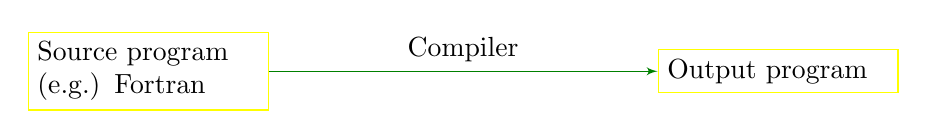
\begin{tikzpicture} [node distance = 8cm, auto]
 \node [rectangle, draw=Yellow, text width=8em] (in) {Source program (e.g.)
 Fortran}; 
 \node [right of=in, rectangle, draw=Yellow, text width=8em] (out) {Output program}; 
 \path [draw=Green, -latex'] (in) -> node {Compiler} (out) ;
\end{tikzpicture}
\end{frame}

\begin{frame}
\frametitle{LLM Compilation}
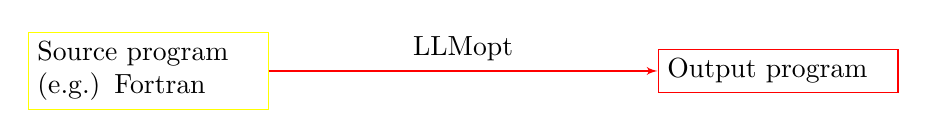
\begin{tikzpicture} [node distance = 8cm, auto]
 \node [rectangle, draw=Yellow, text width=8em] (in) {Source program (e.g.)
 Fortran}; 
 \node [right of=in, rectangle, draw=Red, text width=8em] (out) {Output program}; 
 \path [draw=Red, -latex'] (in) -> node {LLM\supercite{opt}} (out) ;
\end{tikzpicture}
\end{frame}

\begin{frame}
\frametitle{LLM Synthesis}

\begin{tikzpicture} [node distance = 8cm, auto]
 \node [rectangle, draw=Yellow, text width=8em] (in) {Informal \\ Specification}; 
 \node [right of=in, rectangle, draw=Red, text width=8em] (out) {Output program}; 
 \path [draw=Red, -latex'] (in) -> node {LLM\supercite{jigsaw}} (out) ;
\end{tikzpicture}
\end{frame}

\begin{frame}
\frametitle{But I can verify!}
\vspace{2em}
\hspace{3em} \includegraphics[width=0.7\paperwidth]{detective}
\end{frame}

\begin{frame}
\frametitle{Goal}
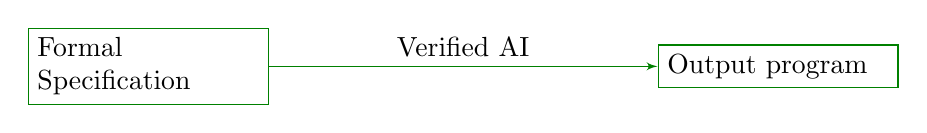
\begin{tikzpicture} [node distance = 8cm, auto]
 \node [rectangle, draw=Green, text width=8em] (in) {Formal \\ Specification}; 
 \node [right of=in, rectangle, draw=Green, text width=8em] (out) {Output program}; 
 \path [draw=Green, -latex'] (in) -> node {Verified AI} (out) ;
\end{tikzpicture}
\end{frame}

\begin{frame}
\frametitle{Motivation}
\includegraphics[width=0.9\paperwidth]{tesla}
\end{frame}

\begin{frame}
\frametitle{Further Reading}
\includegraphics[width=0.4\paperwidth]{deepspec}
\hspace{2em}
\includegraphics[width=0.4\paperwidth]{sf}
\end{frame}

\begin{frame}
\frametitle{ASC/NNSA}
\begin{itemize}[<+->]
\item First NNSA workshop on formal verification to be held in December in Santa Fe.
\item Sandia has been funding this work for at least 10 years, has built expertise.
\item We (LANL) should try and catch up.
\item AI4SS 
\item Come talk to me!
\end{itemize}
\end{frame}

\begin{frame}
\frametitle{References}
\printbibliography
\end{frame}

\end{document}
